%% Genetics in Medicine (GIM) submission -- Original Research Article
%% Marginal Contribution of Cross-Lingual Evidence Extraction to ACMG/AMP
%% Variant Classification: An Ablation Study of a Multi-Agent Literature
%% Curation System
%%
%% Compile:  latexmk -pdf main.tex   (elsarticle.cls is vendored in this dir)
%% Figures:  ../../figures/  (F1-F4; Supplementary Fig. S1 in supplementary.tex)
%% Content reference: ../draft.md; this LaTeX version carries the
%% language-polished submission text (polished 2026-08-13).

\documentclass[preprint,12pt]{elsarticle}

\biboptions{numbers,sort&compress}

\usepackage{amsmath}
\usepackage{amssymb}
\usepackage{booktabs}
\usepackage[hidelinks]{hyperref}

\graphicspath{{../../figures/}}

%% Gentle line-breaking help; long file paths are set with breakable \path.
\emergencystretch=2em

\journal{Genetics in Medicine}

\begin{document}

\begin{frontmatter}

\title{Marginal Contribution of Cross-Lingual Evidence Extraction to
ACMG/AMP Variant Classification: An Ablation Study of a Multi-Agent
Literature Curation System\tnoteref{rt}}
\tnotetext[rt]{Short running title: Cross-lingual evidence for variant
classification.}

%% TODO: replace with the final author list (full names, max two academic
%% degrees per author), affiliations, and corresponding-author details.
\author[aff1]{[Author list TBD]\corref{cor1}}
\cortext[cor1]{Corresponding author: [name, mailing address, telephone,
e-mail: TBD].}
\address[aff1]{[Affiliation TBD]}

\begin{abstract}
Purpose: ACMG/AMP variant classification relies on manual
evidence curation from a predominantly English-language literature,
leaving non-English evidence underused. We quantified the marginal
contribution of cross-lingual evidence extraction.

Methods: Lingua Seeker, a multi-agent four-phase pipeline, processed
thirty ClinGen/ClinVar-curated variant entries in English-only and
dual-track (English plus Chinese translation) modes. A complementary
series of original-language Rett/\textit{MECP2} reports in eight
languages compared English-visible text with native full text using a
frozen ACMG combining rule.

Results: The Chinese track contributed a mean of 3.62 evidence
items per entry that English missed (+22.8\%; $p = 5.9 \times 10^{-6}$);
25/29 entries (86.2\%) gained items. Gold-standard field match was
unchanged (3.57/8; $p = 1.0$). Native full text added ACMG criteria for
20 of 31 case-series events (11 alleles).

Conclusion: Cross-lingual processing adds complementary evidence
without degrading average field-match accuracy. Extra ACMG criteria from
original-language full text measure multilingual contribution more
directly than match against an English-centric gold standard.
\end{abstract}

\begin{keyword}
ACMG/AMP classification \sep variant curation \sep multilingual NLP \sep
large language models \sep multi-agent systems
\end{keyword}

\end{frontmatter}

\section{Introduction}

The ACMG/AMP guidelines define a structured evidence framework for
variant pathogenicity classification, which requires the systematic
curation of genetic and clinical evidence from the biomedical
literature~\cite{richards2015,tavtigian2018,harrison2019}. This curation
process is labor-intensive and dominated by English-language sources, and
language remains a major barrier to the global flow of scientific
evidence~\cite{amano2016}. Existing decision-support tools,
Mastermind~\cite{chunn2020}, ClinVar Miner~\cite{henrie2018}, and
LitVar~\cite{allot2018}, search English-language databases such as
PubMed and ClinVar and do not provide full-text, semantics-aware evidence
extraction, leaving the non-English genetic literature systematically
underutilized. For variants studied primarily in non-English-speaking
populations, this language bias can lead to incomplete evidence bases
and, potentially, to misclassification.

Large language models (LLMs) coupled with multi-agent orchestration can
support automated, language-agnostic evidence curation~\cite{singhal2023}.
However, the clinical value of processing documents in their original
language alongside English translations, rather than in English alone,
has not been quantified. We therefore processed the same 30 variant
entries twice: once with English-only evidence extraction and once with
dual-track extraction from the original English article and a
machine-translated Chinese version. We compared the resulting evidence
yield and field-level match against ClinGen/ClinVar gold-standard ACMG
evidence fields.

We present Lingua Seeker, a multi-agent system for cross-lingual evidence
curation that covers the workflow from literature acquisition to expert
review. We evaluate the system with an ablation design that separates
evidence-item yield from field-level match against a gold standard, and
with a complementary case series of original-language Rett/\textit{MECP2}
reports that asks whether native full text supplies ACMG criteria omitted
from English abstracts and figure legends.

\section{Materials and Methods}

\subsection{System architecture}
\label{sec:architecture}

Lingua Seeker is a multi-agent web server built on an orchestrated
vertical-slice architecture (Figure~\ref{fig:architecture}). A LangGraph
orchestrator coordinates the workflow. The system acquires literature
from more than 15 providers, including Crossref, PubMed, OpenAlex,
EuropePMC, PMC, DOAJ, J-STAGE, Unpaywall, and web scrapers for
CyberLeninka, Hans Publishers, PubScholar, KoreaScience, ChinaXiv, and
Redalyc. MinerU parses PDF documents into markdown while retaining
tables, figures, and layout coordinates~\cite{wang2024mineru}, and Rust
PyO3 extensions accelerate HTTP I/O. The system then performs
cross-lingual dual-track evidence extraction and standardizes entities
against HGNC, OMIM, HPO, and ClinVar through exact and vector-similarity
matching with BAAI bge-m3 embeddings~\cite{chen2024m3} and pgvector. An
expert review workbench provides bidirectional source grounding and a
delta audit log. Typed Pydantic contracts manage pipeline state, and LLM
calls are routed through OpenAI-compatible APIs to models configured for
general-purpose, reasoning, or multimodal tasks.

\begin{figure}[htbp]
  \centering
  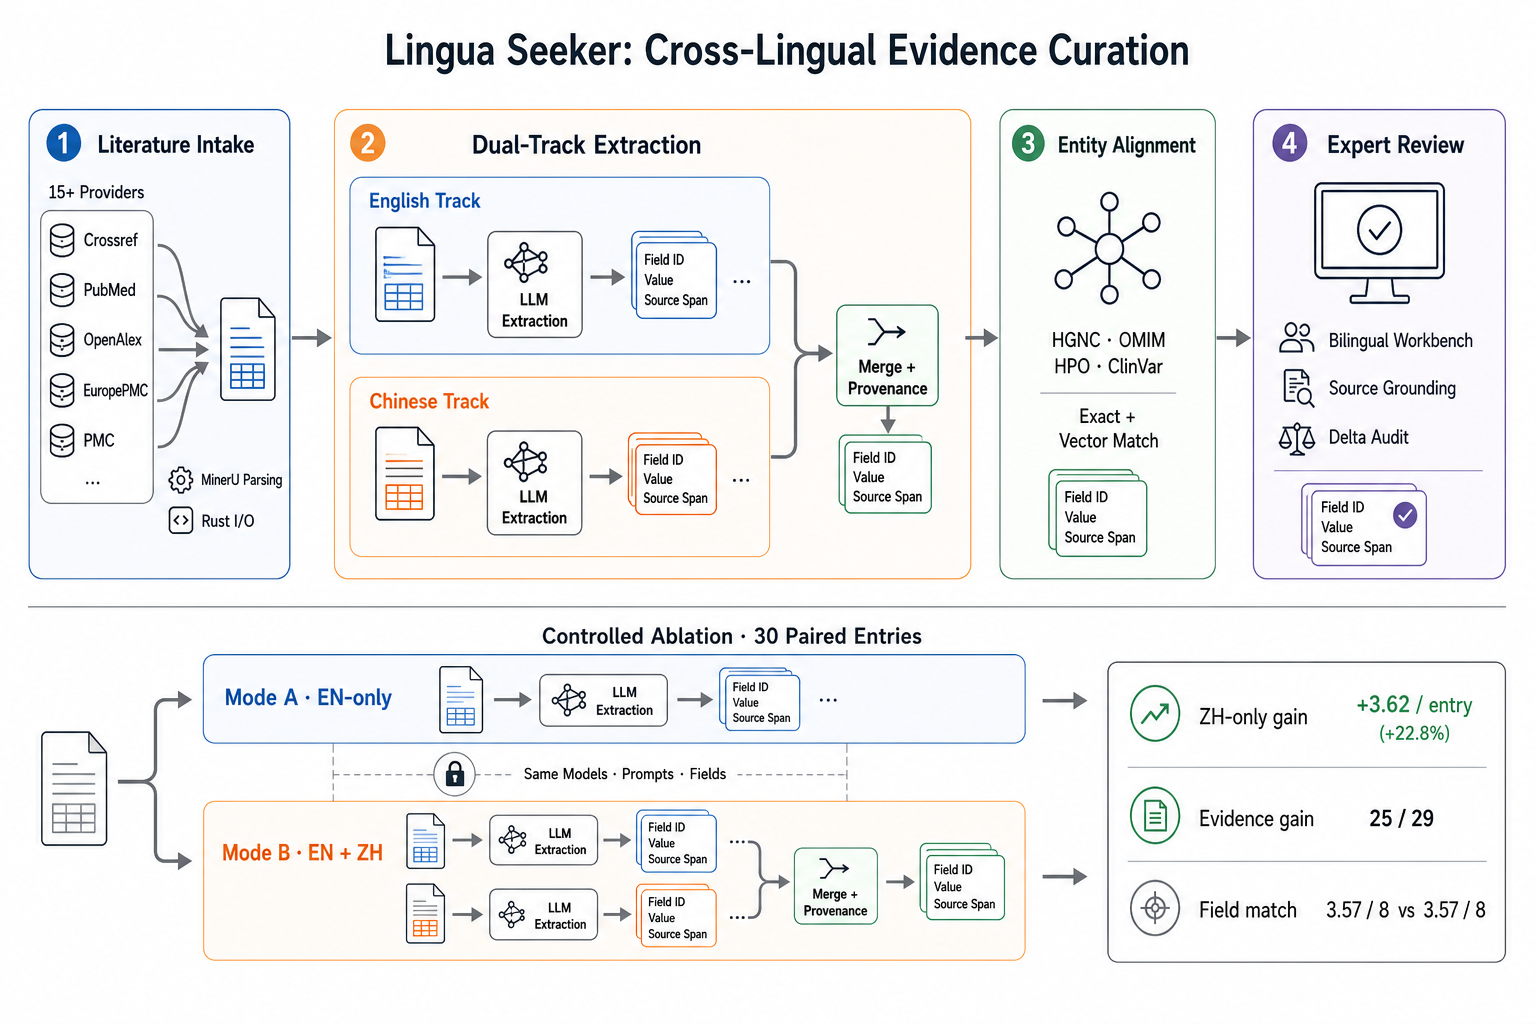
\includegraphics[width=\textwidth]{F1_architecture_redesign.png}
  \caption{The four-phase multi-agent pipeline of Lingua Seeker and the
  controlled ablation design. The top row shows literature acquisition
  and digitization, cross-lingual dual-track evidence extraction, entity
  standardization and knowledge alignment, and expert review. The bottom
  inset compares Mode A (English-only) with Mode B (dual-track, EN + ZH)
  and shows the measured outcomes.}
  \label{fig:architecture}
\end{figure}

\subsection{Cross-lingual dual-track evidence extraction}

For each input document, a language detector determines the source
language. Non-English documents proceed through a multi-stage translation
pipeline that preserves terminology and structure before draft
translation, review, and refinement. Evidence extraction then runs on two
parallel tracks. The native track processes the document in its original
language, while the translated track processes the translated version
(the English translation for non-English source documents). Each track
extracts structured ACMG evidence items (field identifier, value, status,
and source grounding with page and span references) against a catalog of
evidence fields organized into categories A--J, covering gene, variant,
disease/phenotype, inheritance, clinical evidence, and assay information,
among others. Track outputs are grouped and merged, and every evidence
item retains provenance to its source span in the original document.

\subsection{Gold-standard dataset}

We constructed a fused gold-standard set from ClinGen~\cite{rehm2015}
(Definitive or Strong gene--disease assertions) and
ClinVar~\cite{landrum2014} (high-confidence variant classifications),
selecting 75 entries with full-text PMC articles. For the ablation study,
we used 30 of these entries (fused\_000--fused\_029), each annotated with
eight expected ACMG evidence fields: gene symbol, gene--disease
relationship, disease diagnosis, mode of inheritance, variant HGVS c.,
variant HGVS p., variant type, and ClinVar assertion (for fused\_000, for
example: CFTR, cystic fibrosis, causative, AR, c.1521\_1523del,
p.Phe508del, deletion, and Pathogenic). The source articles are
English-language PMC open-access papers, and each entry also carries a
system-generated Chinese translation produced by the multi-stage
translation pipeline, so that the same article is available in both
languages for the dual-track comparison. In this setting, the native
track processes the English original and the translated track processes
the Chinese translation; the two tracks are therefore referred to as the
English track and the Chinese track hereafter.

\subsection{Ablation design}

Each of the 30 entries was run through the pipeline twice. In EN-only
mode (\texttt{ablation\_original\_only=True}), evidence was extracted
only from the English article. In dual-track mode
(\texttt{ablation\_original\_only=False}), evidence was extracted in
parallel from the English and Chinese versions and then merged.

All other parameters, including the models, prompts, and field catalog,
were identical. All runs were executed against the live backend service,
and both runs completed for all 30 entries. All 30 pairs were included in
the field-level match analysis. In one entry (fused\_017), a transient
extraction failure left no evidence items with status ``found'' in either
track of the dual-track run; this entry was excluded from the
evidence-item yield analysis, which therefore covers 29 entries. Per-run
wall-clock durations are reported in Supplementary Note~S4.

\subsection{Evaluation metrics}
\label{sec:metrics}

We measured evidence-item yield within the dual-track runs by counting
items with status ``found'' in each extraction result. EN-track items are
those found in the English track. ZH-only items are those found in the
Chinese track for which the English track found no equivalent; we report
this marginal contribution as both a mean per entry and a percentage of
the EN-track mean. We also report combined unique fields, defined as the
number of distinct field identifiers in the union of the two tracks
after deduplication. This is a field-level count rather than an item-level
count.

For the gold-standard comparison, each of the eight expected fields was
scored as matched or unmatched in each mode. We recorded the number of
matched fields per entry (0--8) and whether each discordant field was
missed under English-only processing but found under dual-track
processing, or vice versa.

\subsection{Statistical analysis}

Per-entry ZH-only item gains (29 valid entries; nonnegative by
construction, with a point mass at zero) were tested against zero with a
one-sided Wilcoxon signed-rank test, and the matched-pairs rank-biserial
correlation $r$ is reported as an effect size. Per-entry matched-field
counts (30 entries) and final-output evidence-item counts were compared
between modes with two-sided Wilcoxon signed-rank tests on the non-zero
differences. Discordant field pairs across the 30 entries $\times$ 8
fields (fields matched under exactly one mode) were tested with the exact
McNemar binomial test. Ninety-five percent confidence intervals (CIs)
were computed with the Wilson score method for proportions and with the
Student $t$ distribution for mean differences. All analyses used SciPy
1.17 under Python 3.12, and the analysis script
\path{benchmark/analysis/gim_statistics.py} reproduces all reported
statistics from the committed reports.

\subsection{LLM configuration}

The general-purpose, reasoning, and multimodal LLM roles were configured
independently and routed by task (extraction and translation;
verification; figure and pedigree parsing). All models were accessed
through OpenAI-compatible endpoints, and no model was shared across
roles. The specific model identifiers are configurable per deployment and
are listed in the repository configuration.

\subsection{Original-language Rett/\textit{MECP2} case series}
\label{sec:case-series}

The ablation corpus uses English PMC articles and machine-generated
Chinese translations. To test whether original non-English full text
supplies ACMG criteria that English abstracts omit, we scored seventeen
published Rett/\textit{MECP2} reports (eight Chinese, two Korean, two
Russian, one Turkish, one Spanish, one Portuguese, one French, one
Japanese) that had been digitized into hashed, reviewed source files.
Thirty-one on-disk variant events from these reports entered the analysis.

For each event we compared two fact sets. The English-visible layer
comprised the author English abstract and any English figure legends. The
native layer used the original-language full text. Scoring on the English
layer required a coding HGVS string in that layer; without it the layer
was recorded as not scorable. Parental testing and diagnosis were counted
in the English layer only when the corresponding fields appeared there.
Variant class and \textit{MECP2} residue position were treated as
properties of the allele, not of language.

A frozen, deterministic rule then granted PM6, PVS1, PP4, or PM1 from
those fields and combined them under the ClinGen Rett/Angelman-like
variant curation specifications~\cite{mcknight2022} and the Richards 2015
pathogenic and likely-pathogenic combinations~\cite{richards2015}. The
extractor does not write ACMG codes. Author-reported strings such as
PS2+PM2+PP3 were not inherited, and PS2 was never granted without
confirmed parentage. The primary endpoint was extra granted criteria
(native codes minus English-visible codes). A change in combining class
is a stronger subset of that endpoint, not a requirement. Reproduction
uses \path{benchmark/experiments/acmg_multilingual/} and the command
\texttt{check-allele-class-increment}. Rule details and the event table
are in Supplementary Note~S6 and Supplementary Table~S3.

\section{Results}

\subsection{Evidence-item yield: multilingual processing adds
complementary evidence}

Across the 29 valid dual-track runs (one entry was excluded because of a
transient pipeline failure), the Chinese track contributed evidence
beyond the English track for most entries
(Figure~\ref{fig:paired}, Figure~\ref{fig:gain}). The
English track found a mean of 15.9 evidence items per entry, and the
Chinese track contributed a mean of 3.62 additional items per entry that
the English track did not find, corresponding to a 22.8\% increase over the
English-track mean (one-sided Wilcoxon signed-rank test, $p = 5.9 \times
10^{-6}$; matched-pairs rank-biserial $r = 0.49$; 95\% CI of the mean
gain, 2.62--4.62 items). Gains occurred in 25/29 entries (86.2\%; 95\%
CI, 69.4\%--94.5\%). After merging, the combined output contained a mean
of 17.24 unique evidence fields per entry (the field-identifier union
across tracks).

In 13/29 entries (44.8\%; 95\% CI, 28.4\%--62.5\%), at least one field
was supported by evidence found only in the Chinese track.

\begin{figure}[htbp]
  \centering
  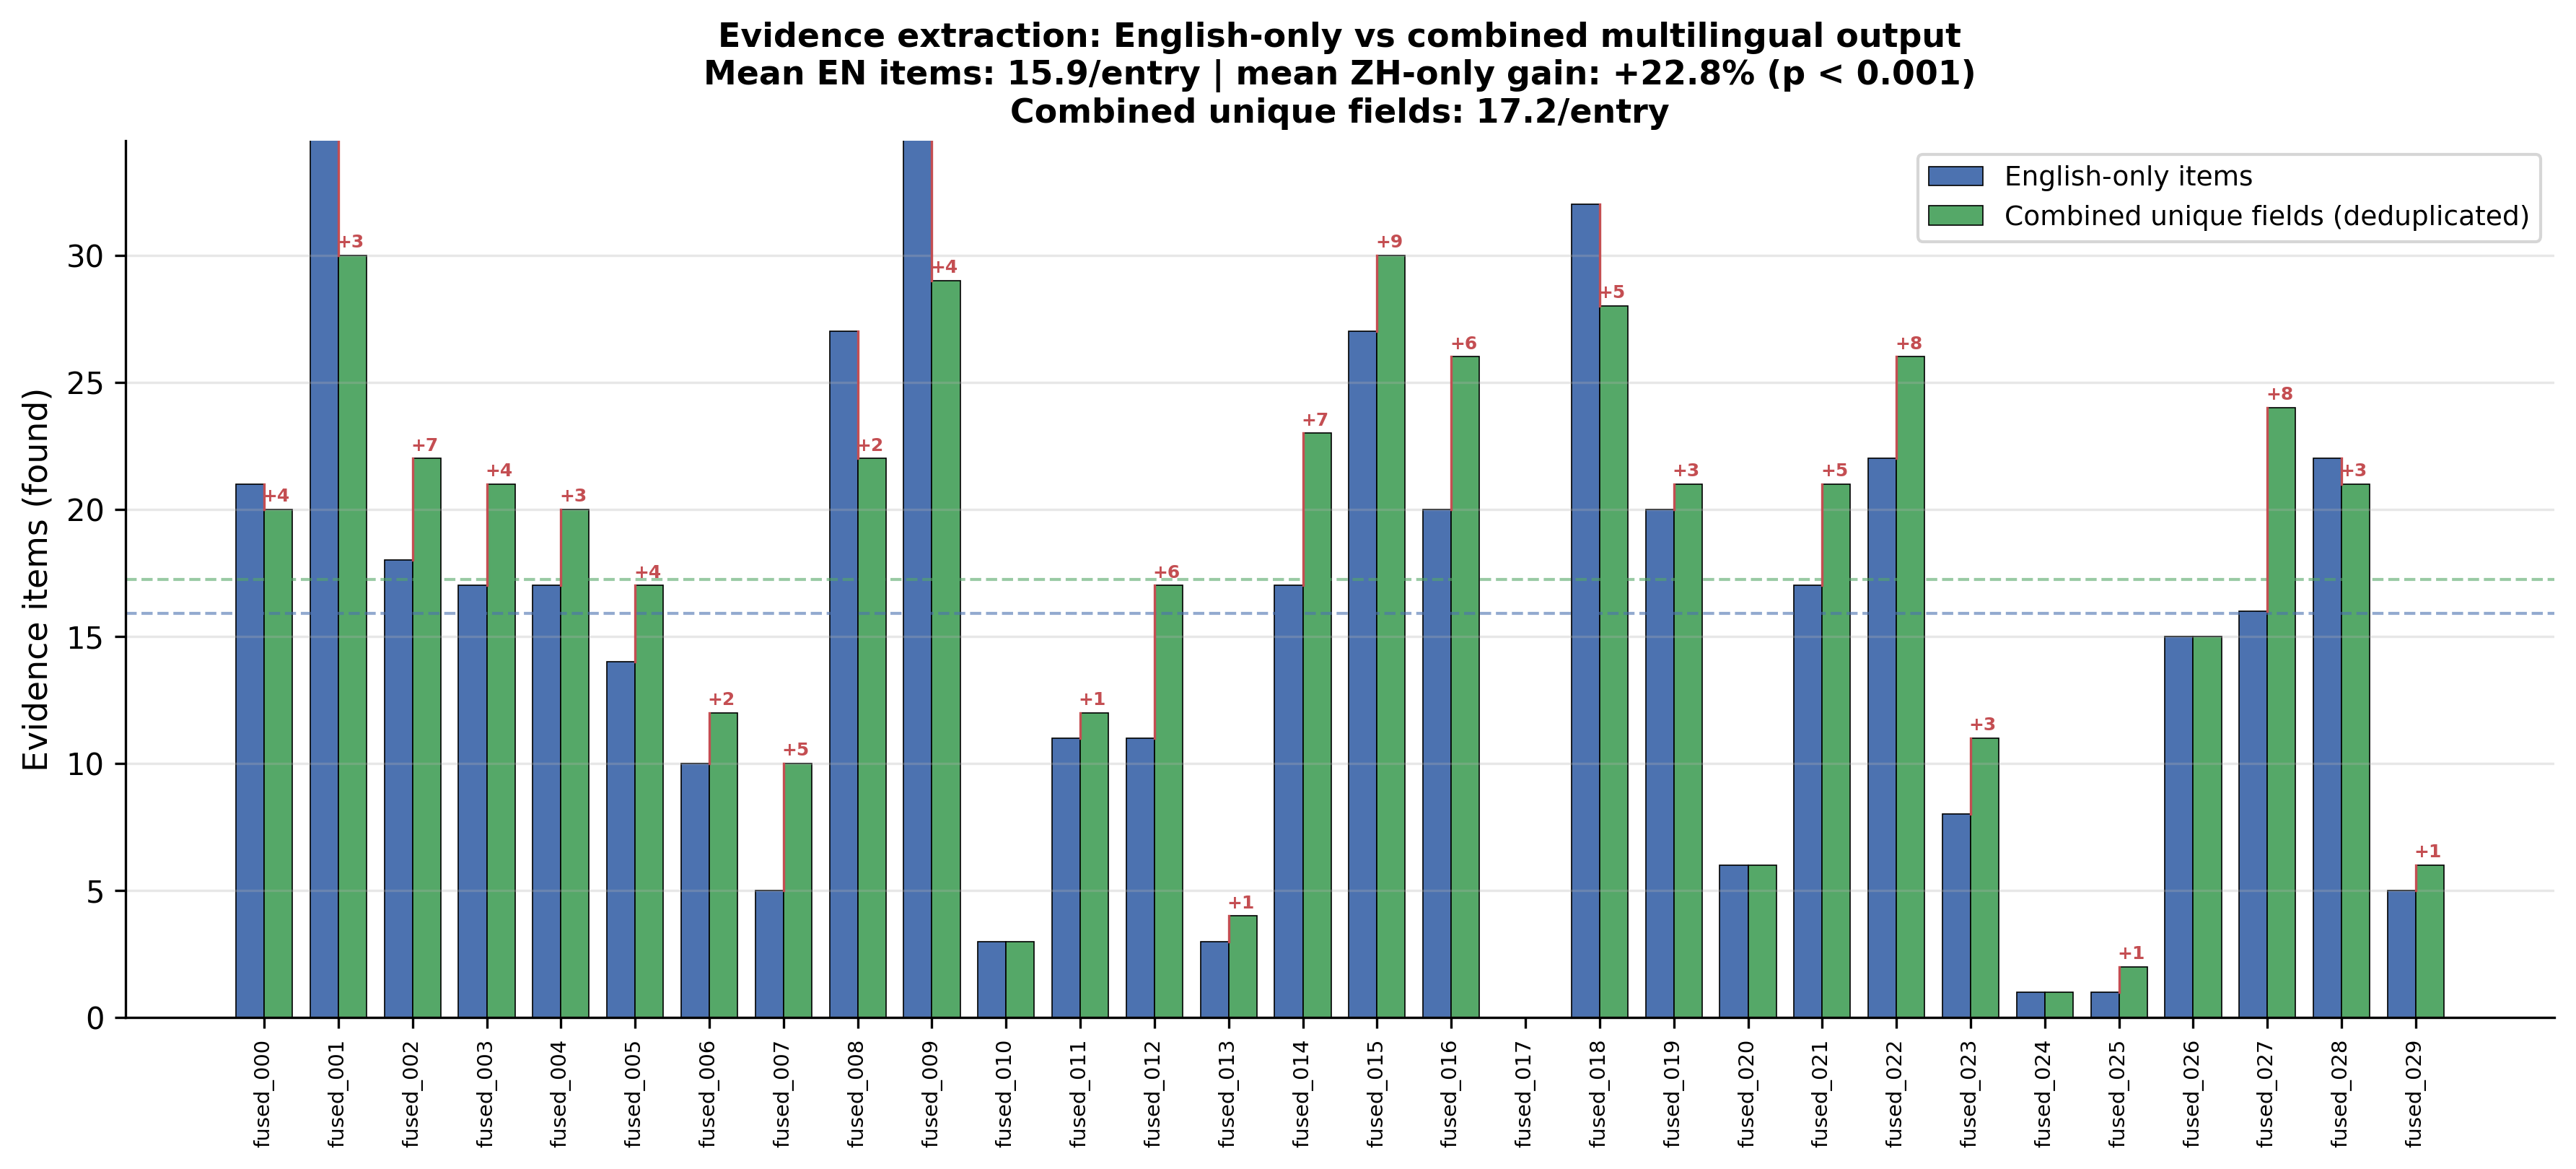
\includegraphics[width=\textwidth]{F2_paired_evidence_comparison.png}
  \caption{Paired per-entry comparison of evidence items found by the
  English-only track and the combined multilingual (EN+ZH) union. Blue
  bars show English-track items, green bars show combined unique fields
  after deduplication (a field-level count; see
  Section~\ref{sec:metrics}), and red connectors mark entries with a
  ZH-only contribution (+$N$ items). The mean English-track yield is
  15.9 items per entry, and the mean ZH-only gain is 3.62 items per
  entry (+22.8\%).}
  \label{fig:paired}
\end{figure}

\begin{figure}[htbp]
  \centering
  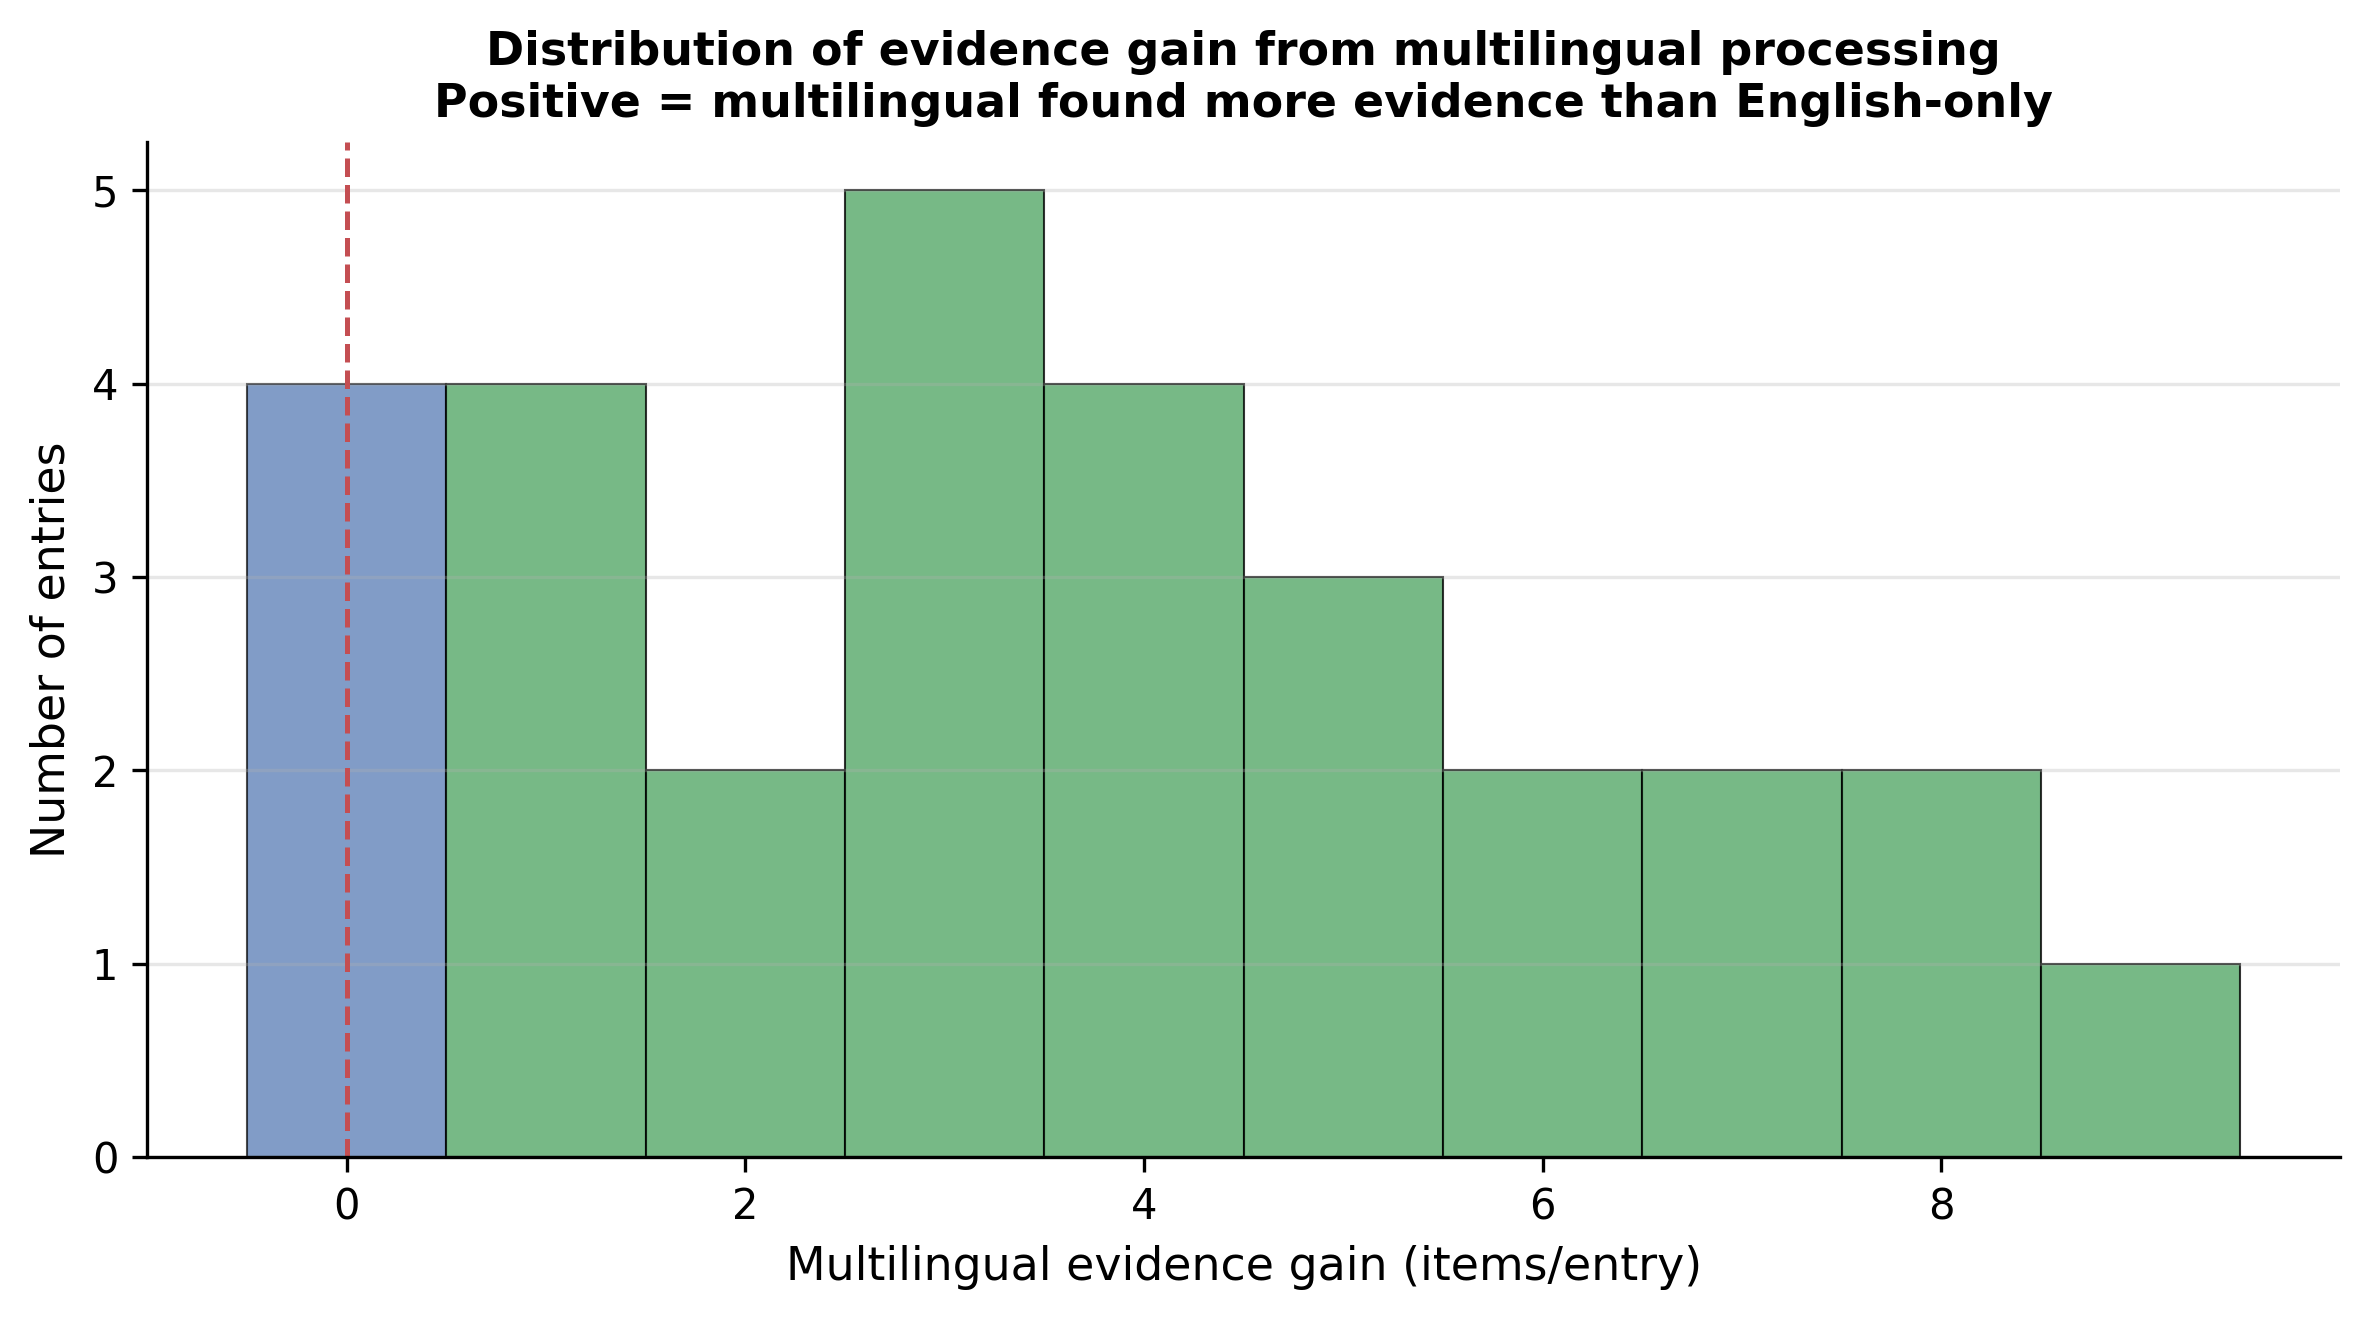
\includegraphics[width=0.85\textwidth]{F3_evidence_gain_distribution.png}
  \caption{Distribution of the per-entry multilingual evidence gain
  (ZH-only items). Twenty-five of 29 entries had a positive gain. Gains
  are nonnegative by construction because the metric counts items found
  only by the Chinese track.}
  \label{fig:gain}
\end{figure}

\subsection{Field-level benefit: which ACMG fields gain from the Chinese
track}

The 23 ZH-only field instances across 13 entries span 14 field types
(Figure~\ref{fig:heatmap}). The most frequently affected fields
were clinical phenotypes (3 entries), assay type (3), ClinVar assertion
(2), HPO terms (2), age of onset (2), disease diagnosis (2), and de novo
status (2); singleton gains occurred for mode of inheritance, inheritance
source, contradiction type, case count, variant consequence class,
functional domain or hotspot, and sex. Fields in category B
(disease/phenotype) and category C (clinical evidence) were most common.
This distribution is consistent with the hypothesis that the English
track extracts some details in Chinese-language clinical descriptions,
including phenotypes, onset, and assay context, incompletely. The total
found items by ACMG category for each track are shown in Supplementary
Figure~S1.

\begin{figure}[htbp]
  \centering
  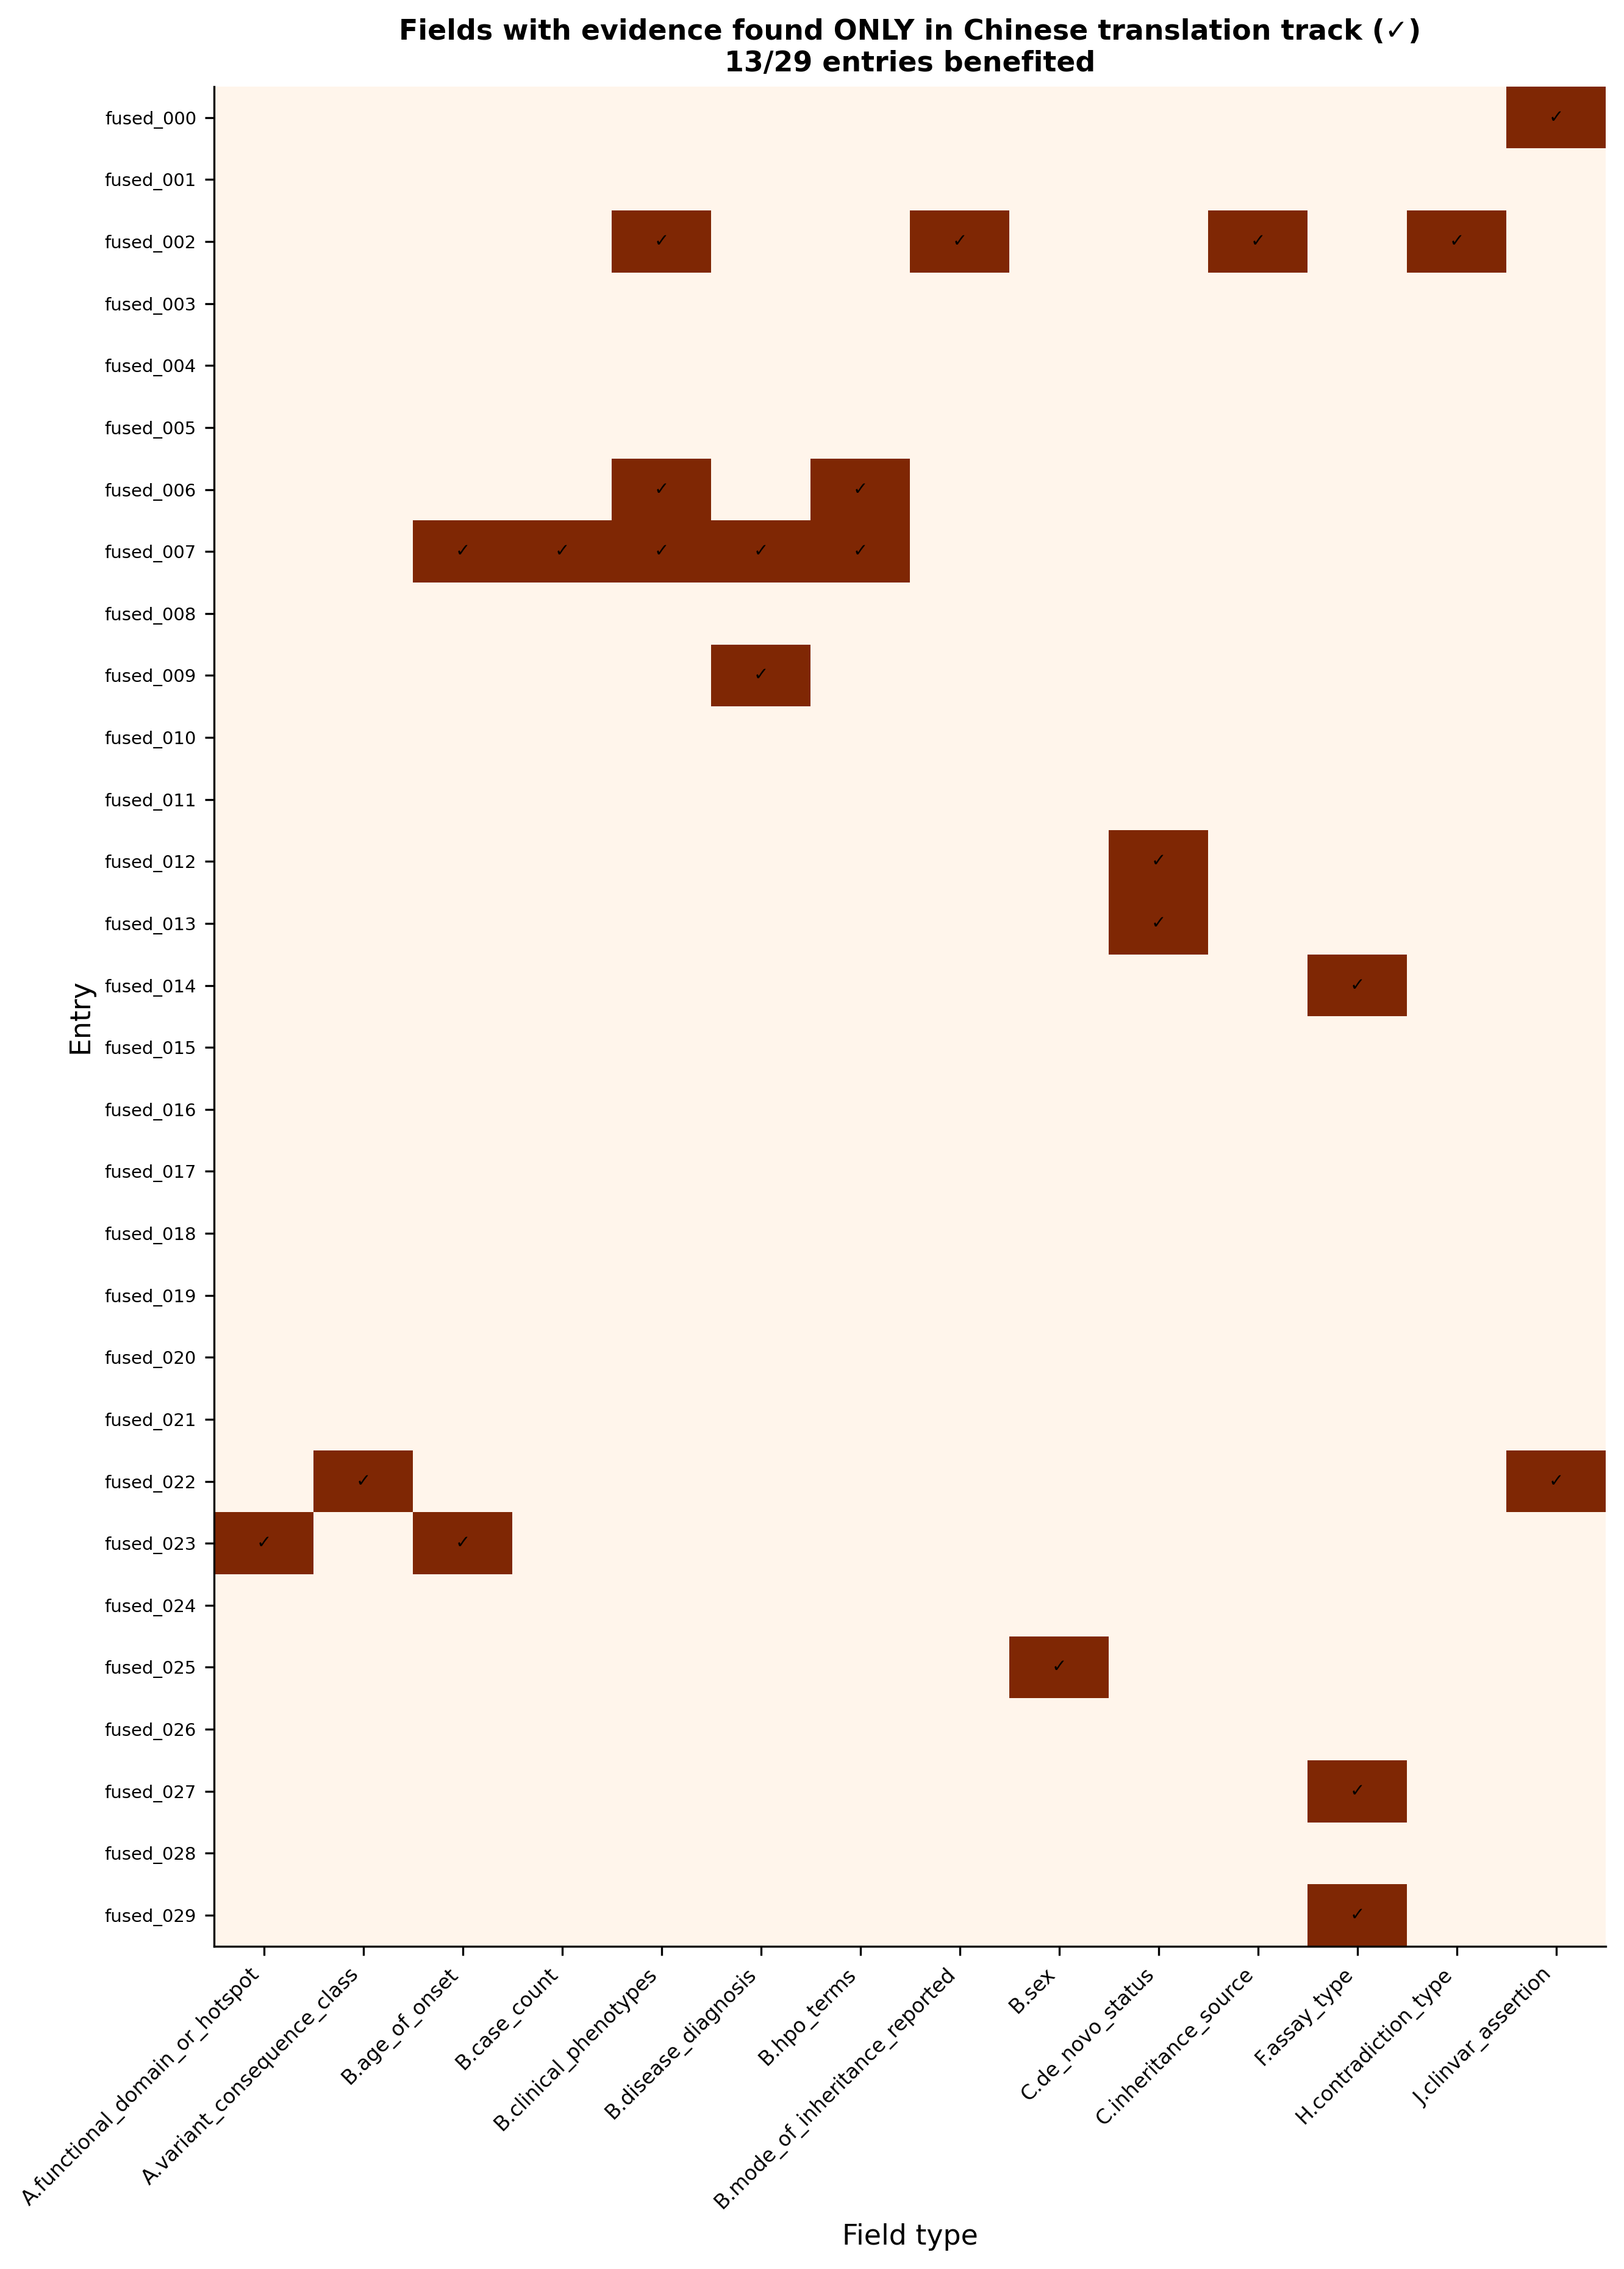
\includegraphics[width=0.9\textwidth]{F4_field_level_zh_benefit_heatmap.png}
  \caption{Heatmap of entries (rows) $\times$ field types (columns);
  \checkmark{} marks fields with evidence found only in the Chinese
  track. Overall, 13/29 entries show at least one ZH-only field.}
  \label{fig:heatmap}
\end{figure}

\subsection{Field-match ablation: no average change, occasional rescues}

Against the eight-field gold standard, the two modes achieved an
identical mean of 3.57 matched fields per entry
(Table~\ref{tab:summary}; mean difference, 0.000; 95\% CI,
$-0.139$ to $+0.139$; two-sided Wilcoxon signed-rank test on the non-zero
differences, $p = 1.0$). Per-field discordance was symmetric: three
fields were matched only under dual-track processing and three only under
English-only processing (exact McNemar test, $p = 1.0$). The per-entry
changes clarify this result: 3/30 entries (10\%) gained at least one field
match under dual-track processing, and 3/30 lost at least one. One entry
(fused\_016) did both, exchanging one field for another. In net terms,
two entries improved, two regressed, and 26 were unchanged
(Table~\ref{tab:summary}, Supplementary Table~S1).

In fused\_005 (ADA), dual-track processing recovered the variant type
``missense,'' which English-only processing had missed. In fused\_024
(GP1BA), it recovered the gene symbol: this entry had no matched fields
under English-only processing (0/8) but matched GP1BA under dual-track
processing (1/8). In fused\_016 (DNM2), the Chinese track recovered the
mode of inheritance (``autosomal dominant'') but lost the gene-disease
relationship field.

Two further entries lost fields under dual-track processing:
fused\_022 (GJB2) lost the disease diagnosis, and fused\_028 (HBB) lost
the variant HGVS c.\ annotation. In
both cases, the merged output dropped a field that the English track had
found. These losses are a potential signal of merge and consolidation
artifacts and are addressed in the Discussion.

\subsection{Summary of ablation results}

\begin{table}[htbp]
  \centering
  \caption{Ablation outcomes for the 30 ClinGen/ClinVar entries processed
  under the English-only and dual-track modes. Track-level items are
  measured within dual-track runs (English-track items vs.\ ZH-only
  items), whereas field matches are measured against the eight-field gold
  standard for each mode. The gain and loss rows count entries with at
  least one changed field; the swap entry (fused\_016) appears in both
  counts.}
  \label{tab:summary}
  \small
  \begin{tabular}{@{}p{5.8cm}p{1.8cm}p{4.6cm}@{}}
    \toprule
    Metric & EN-only & Dual-track (EN+ZH) \\
    \midrule
    Valid paired comparisons & NA & 30/30 \\
    Mean matched fields / entry (of 8) & 3.57 & 3.57 (diff 0.000; $p = 1.0$) \\
    Mean evidence items in final output / entry & 109.9 & 99.7 ($-10.2$; $p = 0.27$) \\
    Entries gaining $\geq$1 field match & NA & 3/30 (10\%) \\
    Entries losing $\geq$1 field match & NA & 3/30 (10\%) \\
    \quad of which: net gain / net loss / swap ($\pm$0) & NA & 2 / 2 / 1 \\
    Mean evidence items, track level (EN track vs.\ ZH-only) & 15.9 & 3.62 ZH-only (+22.8\%; $p = 5.9 \times 10^{-6}$) \\
    Entries with track-level evidence gain & NA & 25/29 (86.2\%) \\
    Entries with ZH-only evidence fields & NA & 13/29 (44.8\%) \\
    \bottomrule
  \end{tabular}
\end{table}

\subsection{Original-language reports: extra ACMG criteria}

Across 31 on-disk events from 17 original-language reports in eight
languages, native full text granted ACMG criteria that the English-visible
layer did not for 20 events spanning 11 alleles (Supplementary Table~S3).
Four of those twenty events came from one Chinese series whose English
abstract described genetic testing of the children and parents but did
not list per-case HGVS strings or parental negatives~\cite{liu2023}. After
excluding that series, sixteen events remained. A missense allele gained
only PM6 and stayed evidence-insufficient~\cite{zhong2024}. A nonsense
allele gained PVS1+PM6+PP4 and reached Pathogenic~\cite{han2022}. A
Russian report whose English abstract named a \textit{MECP2} mutation but
not the HGVS string gained PP4+PM1 for p.Asp156Glu and stayed
evidence-insufficient~\cite{kovalenkova2025}. The matching Chinese report
on that allele supplied parental negatives and gained PM6+PP4+PM1, still
insufficient~\cite{hu2017}. A Korean cohort table that the English
abstract did not itemize added the same p.Asp156Glu allele, plus T158M and
R168X~\cite{park2002}. A Japanese cohort table likewise named D156E,
T158M, and R168X as protein symbols without coding HGVS~\cite{kondo2002}.
A French conference poster with no English abstract
added R106W, R168X, and R255X~\cite{ghorbel2018}. A Turkish report whose
English abstract omitted HGVS gained PP4+PM1 for
p.Pro302Leu~\cite{aydin2015}. A truncating allele without parental testing
gained PVS1+PP4 and also stayed insufficient~\cite{yang2018}. The same
T170M nucleotide as in the Liu series was maternal in a separate Chinese
report: the engine granted PP4 from the diagnosis and refused
PM6~\cite{li2026}. Spanish and Portuguese reports were negative controls:
their English abstracts already named \texttt{c.806del} and
\texttt{c.763C}\textgreater\texttt{T}~\cite{cote2023,reiner2021}. A second
Russian report on p.Asp156Glu was likewise a negative control: its English
abstract already named \texttt{c.468C}\textgreater\texttt{G}~\cite{burlutskaya2021}.

The missense example counts as a gain on the primary endpoint. The English
abstract already supported PP4 (Rett diagnosis). The Chinese text stated
that neither parent carried \texttt{c.710C}\textgreater\texttt{G}. The rule granted PM6 at
Moderate strength, refused the authors' PS2+PM2+PP3 string, and left the
combining class as evidence-insufficient because p.Pro237Arg (e2
p.Pro225Arg) lies outside the VCEP methyl-CpG-binding and transcriptional
repression residues used for PM1. ClinVar already classifies this allele
as Pathogenic from other evidence. Extra criterion evidence is therefore
not the same as a class flip and not the same as a new database
assertion.

Four events reached Pathogenic from an English-visible layer that was not
scorable (three truncating alleles in the Liu series and R168X in Han et
al.). Those alleles already have ClinVar Pathogenic records. Two further
alleles, \texttt{c.913insT}~\cite{zhao2014} and
\texttt{c.194delC}~\cite{ge2018}, were Pathogenic from the English abstract
already (PVS1+PM6+PP4) and have no exact ClinVar VCV; \texttt{c.194delC} is
adjacent to, not identical with, VCV001076185. No event was both an
English-visible increment and a ClinVar-gap Pathogenic call. The Korean
report's English figure legend already recorded patient-only occurrence
of \texttt{c.455C}\textgreater\texttt{G}, so the native text added no criteria~\cite{kim2002}. One
ClinVar expert-panel Benign missense (p.Pro376Ser) was blocked despite
recovered parental negatives.

\section{Discussion}

Processing the Chinese translation alongside the English original added
evidence for 86\% of entries, with a mean increase of 22.8\% in unique
evidence items. It also recovered the variant type, mode of inheritance,
or gene symbol for 10\% of entries, while the mean gold-standard field
match remained unchanged. To our knowledge, this is the first
quantitative estimate of the marginal contribution of cross-lingual
evidence extraction to ACMG/AMP variant classification.

The original-language case series asks a different question: whether
native full text supplies ACMG criteria that the English-visible layer of
the same PDF omits. In 20 of 31 events it did. The increment is extra
granted criteria, not a required Pathogenic flip. The Zhong et al.\
missense, which gained only PM6 and remained evidence-insufficient, is a
positive result on that endpoint, as are the Russian, Korean, Japanese,
and French reports that named a coding change only in the native layer. Four events
did reach Pathogenic once the native text supplied HGVS and parental
negatives, but those alleles are already Pathogenic in ClinVar. The two
alleles without an exact ClinVar VCV were already Pathogenic from their
English abstracts. A maternal T170M report shows why de novo cannot be
inferred from the nucleotide alone. We did not recover a Pathogenic
combining class that was missing from both the English-visible layer and
ClinVar.

The difference between evidence yield and field-level match partly
reflects the composition of the gold standard. ClinGen/ClinVar assertions
and their supporting evidence are derived from the English-language
literature. Clinical phenotypes and age of onset, two areas in which the
Chinese track contributed evidence, are not part of the eight-field match
set. Instead, the set contains several language-invariant fields,
including gene symbols and HGVS nomenclature. Evidence yield is therefore
more sensitive to multilingual contributions, whereas an English-centric
gold standard may understate the field-level utility of non-English
literature.

Entry fused\_024 (GP1BA) progressed from a
complete failure (0/8 fields) under English-only processing to 1/8 under
dual-track processing. Such failures are problematic in clinical
workflows because they are indistinguishable from an absence of evidence.
Of the two entries with no matched fields under English-only processing,
the Chinese track recovered one field for fused\_024; fused\_017 had no
matched fields under either mode.

Three entries lost a field under
dual-track processing (one as part of a swap). At the item level, the
final outputs of dual-track runs contained numerically fewer evidence
items than those of English-only runs (99.7 vs.\ 109.9 per entry),
although this difference was not statistically significant (95\% CI,
$-30.6$ to $+10.3$; $p = 0.27$). These losses appear to arise from the
current consolidation step, which can drop items when it merges the two
tracks. A field-level arbitration procedure could reduce this problem.
The present implementation uses a first-found-wins policy with
provenance; future versions could arbitrate conflicts with an LLM.

For variants whose evidence appears mainly in Chinese-language
publications, an English-only workflow may miss relevant reports.
Processing translated versions of the same articles can reduce this
language bias without requiring a separate literature search.

This study has several limitations. The ablation corpus consists of
English PMC articles paired with machine-generated Chinese translations.
The original-language case series uses published Rett/\textit{MECP2}
reports in eight languages rather than translations, but it is still
small (seventeen reports, 31 events), still dominated by Chinese sources,
and scored with a frozen Stage-0 combining rule rather than blinded
laboratory ACMG assignment. A hashed Japanese cohort supplies protein
symbols without named-proband parental genotypes~\cite{kondo2002}; other
owned Japanese files are a review or FOXG1/CDKL5 papers. Open-access
German \textit{MECP2} point-variant case reports that could be hashed
were not located (the 2002 Leipzig series is paywalled; congress slides
redacted the variant). Four of the twenty extra-criterion events come from one case series, so event
counts overstate the number of independent publications. The product extraction pipeline still does not
write ACMG codes. Field-level match in the ablation was measured against
only eight fields from the catalog. The evaluation also used one LLM
family and a sample of 30 ablation entries, so performance may differ
with other models and the estimated 10\% rescue rate remains uncertain.

Cross-lingual dual-track evidence extraction
contributes complementary, clinically relevant evidence for most variants
and occasionally rescues failed extractions, without degrading average
gold-standard performance. In original-language Rett/\textit{MECP2}
reports, native full text can add ACMG criteria that English abstracts
and figure legends omit, including a Moderate de novo criterion that does
not by itself change combining class. These findings support the use of
multilingual processing in ACMG evidence curation, particularly when the
supporting literature includes non-English articles.

\section*{Data Availability}

The source code of Lingua Seeker is available at
\url{https://github.com/lanshi17/LinguaSeeker} (branch
\texttt{feature/gim-submission}). All ablation reports and per-entry
results underlying the reported statistics are committed in the
repository under \path{docs/gim/supplementary/reports/} (mirrored from
the runner output directory \path{benchmark/data/reports/nar_ablation/}):
\path{ablation_report.json} (field-match ablation),
\path{multilingual_contribution_report.json} (evidence-item yield),
and \path{en_only_metrics.json}/\path{dual_track_metrics.json}
(per-mode final outputs and wall-clock durations). The analysis scripts
(\path{benchmark/analysis/gim_statistics.py},
\path{benchmark/analysis/generate_gim_figures.py},
\path{benchmark/analysis/generate_gim_architecture.py}) reproduce all
statistics, Figures~\ref{fig:architecture}--\ref{fig:heatmap}, and
Supplementary Figure~S1 from these reports; Supplementary Figure~S1
additionally requires the per-run pipeline outputs, which are available
from the authors on request because of their size. Hashed source files
and the frozen event table for the original-language Rett/\textit{MECP2}
case series are in
\path{benchmark/experiments/acmg_multilingual/reviewed/} and
\path{benchmark/experiments/acmg_multilingual/direct_inference_cases.json};
the command \texttt{check-allele-class-increment} reproduces
Supplementary Table~S3. The source article corpus consists of PMC
open-access articles, and the Chinese translations
were machine-generated by the translation pipeline of the system. The
original-language case reports are previously published journal
articles. The
gold-standard annotations were curated from ClinGen and ClinVar public
data. External model-inference services (embedding, reranking, and
document parsing) are separate deployments and are not required to
reproduce the reported statistics.

\section*{Acknowledgments}

[TBD]

\section*{Funding Statement}

[TBD: list funders and grant numbers, or state: ``This study received
no specific funding.'']

\section*{Author Contributions}

[TBD: complete with the final author list using the CRediT taxonomy,
e.g.: Conceptualization: A.B.; Data curation: A.B., C.D.; Formal analysis:
A.B.; Funding acquisition: E.F.; Investigation: A.B., C.D.; Methodology:
A.B.; Software: A.B., C.D.; Supervision: E.F.; Validation: C.D.;
Visualization: A.B.; Writing, original draft: A.B.; Writing, review \&
editing: A.B., C.D., E.F.]

\section*{Ethics Declaration}

This study analyzed only publicly available data: gene--disease validity
assertions and variant classifications from ClinGen and ClinVar,
open-access articles from PubMed Central, and previously published
original-language Rett/\textit{MECP2} reports in Chinese, Korean,
Russian, Turkish, Spanish, Portuguese, French, and Japanese. No human participants were
recruited, and no individual-level or identifiable human data were
collected or processed. Institutional Review Board or Research Ethics
Committee review and informed consent were therefore not required.

\section*{Conflict of Interest}

The authors declare no conflict of interest.

\section*{Declaration of AI and AI-assisted technologies in the writing
process}

During the preparation of this work the authors used [name of
tool/service: to be confirmed by the authors] to assist with drafting
and editing the manuscript text. After using this tool/service, the
authors reviewed and edited the content as needed and take full
responsibility for the content of the publication.

\begin{thebibliography}{23}
\providecommand{\natexlab}[1]{#1}
\providecommand{\url}[1]{\texttt{#1}}

\bibitem{richards2015}
Richards S, et al.
\newblock Standards and guidelines for the interpretation of sequence
  variants: a joint consensus recommendation of the American College of
  Medical Genetics and Genomics and the Association for Molecular
  Pathology.
\newblock \emph{Genet Med}. 2015;17(5):405--424.
\newblock doi:10.1038/gim.2015.30.

\bibitem{tavtigian2018}
Tavtigian SV, et al.
\newblock Modeling the ACMG/AMP variant classification guidelines as a
  Bayesian classification framework.
\newblock \emph{Genet Med}. 2018;20(9):1054--1060.
\newblock doi:10.1038/gim.2017.210.

\bibitem{harrison2019}
Harrison SM, et al.
\newblock Overview of specifications to the ACMG/AMP variant
  interpretation guidelines.
\newblock \emph{Curr Protoc Hum Genet}. 2019;103(1):e93.
\newblock doi:10.1002/cphg.93.

\bibitem{amano2016}
Amano T, et al.
\newblock Languages are still a major barrier to global science.
\newblock \emph{PLoS Biol}. 2016;14(12):e2000933.
\newblock doi:10.1371/journal.pbio.2000933.

\bibitem{chunn2020}
Chunn LM, et al.
\newblock Mastermind: a comprehensive genomic association search engine
  for empirical evidence curation and genetic variant interpretation.
\newblock \emph{Front Genet}. 2020;11:577152.
\newblock doi:10.3389/fgene.2020.577152.

\bibitem{henrie2018}
Henrie A, et al.
\newblock ClinVar Miner: demonstrating utility of a web-based tool for
  viewing and filtering ClinVar data.
\newblock \emph{Hum Mutat}. 2018;39(8):1051--1060.
\newblock doi:10.1002/humu.23555.

\bibitem{allot2018}
Allot A, et al.
\newblock LitVar: a semantic search engine for linking genomic variant
  data in PubMed and PMC.
\newblock \emph{Nucleic Acids Res}. 2018;46(W1):W530--W536.
\newblock doi:10.1093/nar/gky355.

\bibitem{singhal2023}
Singhal K, et al.
\newblock Large language models encode clinical knowledge.
\newblock \emph{Nature}. 2023;620(7972):172--180.
\newblock doi:10.1038/s41586-023-06291-2.

\bibitem{wang2024mineru}
Wang B, et al.
\newblock MinerU: an open-source solution for precise document content
  extraction.
\newblock Preprint. arXiv:2409.18839; 2024.

\bibitem{chen2024m3}
Chen J, et al.
\newblock M3-Embedding: multi-linguality, multi-functionality,
  multi-granularity text embeddings through self-knowledge distillation.
\newblock Preprint. arXiv:2402.03216; 2024.

\bibitem{rehm2015}
Rehm HL, et al.
\newblock ClinGen --- the Clinical Genome Resource.
\newblock \emph{N Engl J Med}. 2015;372(23):2235--2242.
\newblock doi:10.1056/NEJMsr1406261.

\bibitem{landrum2014}
Landrum MJ, et al.
\newblock ClinVar: public archive of relationships among sequence
  variation and human phenotype.
\newblock \emph{Nucleic Acids Res}. 2014;42(D1):D980--D985.
\newblock doi:10.1093/nar/gkt1113.

\bibitem{mcknight2022}
McKnight D, et al.
\newblock Recommendations by the ClinGen Rett/Angelman-like expert panel
  for gene-specific variant interpretation methods.
\newblock \emph{Hum Mutat}. 2022;43(8):1097--1113.
\newblock doi:10.1002/humu.24302.

\bibitem{liu2023}
Liu W, Jiang X, You Y, Qin Z, Han Q, Yuan Z.
\newblock Gene mutation analysis of 5 children with Rett syndrome-like
  phenotype.
\newblock \emph{Chin J Birth Health Hered}. 2023.
\newblock doi:10.13404/j.cnki.cjbhh.2023.04.008.

\bibitem{zhong2024}
Zhong S, Li C, Wang Y, Rong S, Liu L, Lin Y, Ao D.
\newblock Clinical phenotype and genetic analysis of one child with Rett
  syndrome caused by \textit{MECP2} gene variants.
\newblock \emph{China Med Herald}. 2024.
\newblock doi:10.20047/j.issn1673-7210.2024.05.45.

\bibitem{han2022}
Han J, Zhou X, Li X, Zhu H, Li J, Xu B.
\newblock A case report of Rett syndrome.
\newblock \emph{J Dalian Med Univ}. 2022;44(6):573--576.
\newblock doi:10.11724/jdmu.2022.06.20.

\bibitem{zhao2014}
Zhao PW, He XL, Lin J, Wu GF, Yue X, Bi B, Hu JS, Liu ZS.
\newblock Clinical features and \textit{MECP2} mutations in children with
  Rett syndrome.
\newblock \emph{Chin J Contemp Pediatr}. 2014;16(4):393--396.
\newblock doi:10.7499/j.issn.1008-8830.2014.04.017.

\bibitem{ge2018}
Ge J, Lan X, Li H, Zhang R, Shen L.
\newblock Report of a boy with Rett syndrome caused by a novel
  \textit{MECP2} mutation and literature review.
\newblock \emph{J Clin Pediatr}. 2018;36(11):824.
\newblock doi:10.3969/j.issn.1000-3606.2018.11.005.

\bibitem{kim2002}
Kim JK, Ki CS, Kim JW.
\newblock A case of Rett syndrome with \textit{MECP2} gene mutation.
\newblock \emph{J Korean Pediatr Soc}. 2002;45:540--544.

\bibitem{kovalenkova2025}
Kovalenkova EA, Kovalenkova SA, Krutikov DS.
\newblock Clinical case of Rett syndrome: the experience of observing an
older preschooler.
\newblock \emph{Pediatricheskaya Farmakologiya}. 2025;22(2):184--188.
\newblock doi:10.15690/pf.v22i2.2872.

\bibitem{burlutskaya2021}
Burlutskaya AV, Ivanenko AS, Statova AV.
\newblock Rett syndrome: a clinical case.
\newblock \emph{Kubanskii Nauchnyi Meditsinskii Vestnik}. 2021;28(1):116--124.
\newblock doi:10.25207/1608-6228-2021-28-1-116-124.

\bibitem{yang2018}
Yang ZL, Jin ZY.
\newblock Rett syndrome: one case.
\newblock \emph{J Med Sci Yanbian Univ}. 2018.
\newblock doi:10.16068/j.1000-1824.2018.01.01.

\bibitem{li2026}
Li WM.
\newblock A male infant with Rett syndrome caused by an \textit{MECP2}
missense variant: one case.
\newblock \emph{J Jilin Med Coll}. 2026.
\newblock doi:10.3969/j.issn.1673-1492.2026.08.016.

\bibitem{hu2017}
Hu T, Li BX, Zhang ZH, Liu GS.
\newblock Rett syndrome: one case and a novel \textit{MECP2} mutation.
\newblock \emph{Clinical Focus}. 2017;32(11):995--997.
\newblock doi:10.3969/j.issn.1004-583X.2017.11.020.

\bibitem{aydin2015}
Ayd{\i}n H, Kabaku\c{s} N, Erko\c{c}o\u{g}lu M.
\newblock Association of atypical Rett syndrome and autism.
\newblock \emph{Sakarya Med J}. 2015;5(4):228--231.
\newblock doi:10.5505/sakaryamedj.2015.08760.

\bibitem{cote2023}
Cote-Orozco JE, Mart{\'\i}nez-C{\'o}rdoba N, Lince-Rivera I,
C{\'o}rdoba-Gravini JL.
\newblock Rett syndrome in a male infant with a pathogenic variant in
\textit{MECP2}.
\newblock \emph{Rev Mex Pediatr}. 2023;90(4):156--161.
\newblock doi:10.35366/114766.

\bibitem{reiner2021}
Reiner GL, Vignardi D, Klingelfus FS, Nath M, Santos PSO.
\newblock Rett syndrome --- rare case report.
\newblock \emph{Arq Catarin Med}. 2021;50(2):363--367.
\newblock doi:10.63845/c3q7eb11.

\bibitem{ghorbel2018}
Ghorbel R, Ghorbel R, Rouissi A, Triki C, Keskes Ammar L, Fakhfakh F.
\newblock Genetic study of Rett syndrome in the Tunisian population:
identification of three hotspot mutations in \textit{MECP2}.
\newblock Poster presented at: 35th Congress of the Soci{\'e}t{\'e} Fran{\c{c}}aise
d'Endocrinologie; 2018 Sep 12--15; Nancy, France.

\bibitem{park2002}
Park SJ, Hwang TG, Son BH, Kim CM.
\newblock Mutational analysis of \textit{MECP2} gene in 34 Rett syndrome.
\newblock \emph{J Korean Pediatr Soc}. 2002;45:1263--1272.

\bibitem{kondo2002}
Kondo I, Yamagata H.
\newblock Mutation spectrum and genotype-phenotype correlation of \textit{MECP2}
in patients with Rett syndrome.
\newblock \emph{No To Hattatsu}. 2002;34:219--223.

\end{thebibliography}

\end{document}
